\documentclass[12pt]{article}
\usepackage[english]{babel}
\usepackage[utf8x]{inputenc}
\usepackage{amsmath}
\usepackage{hyperref}
\usepackage{graphicx}
\usepackage{graphicx, lipsum,caption}
\usepackage[colorinlistoftodos]{todonotes}
\usepackage{caption}
\usepackage{subcaption}
\usepackage{framed}
\usepackage{float}

\begin{document}
	
	\begin{titlepage}
		
		\newcommand{\HRule}{\rule{\linewidth}{0.5mm}} % Defines a new command for the horizontal lines, change thickness here
		
		\center % Center everything on the page
		
		%----------------------------------------------------------------------------------------
		%	HEADING SECTIONS
		%----------------------------------------------------------------------------------------
		
		\textsc{\LARGE Portland State University}\\[1.5cm] % Name of your university/college
		\textsc{\Large Deep Learning: Computational Structures and Programming}\\[0.5cm] % Major heading such as course name
		\textsc{\large Winter 2021}\\[0.5cm] % Minor heading such as course title
		
		%----------------------------------------------------------------------------------------
		%	TITLE SECTION
		%----------------------------------------------------------------------------------------
		
		\HRule \\[0.4cm]
		{ \huge \bfseries Project \#5}\\[0.4cm] % Title of your document
		\HRule \\[1.5cm]
		
		%----------------------------------------------------------------------------------------
		%	AUTHOR SECTION
		%----------------------------------------------------------------------------------------
		
		\begin{minipage}{0.4\textwidth}
			\begin{flushleft} \large
				\emph{Author:}\\
				Hermann \textsc{Yepdjio} % Your name
			\end{flushleft}
		\end{minipage}
		~
		\begin{minipage}{0.4\textwidth}
			\begin{flushright} \large
				\emph{Professor:} \\
				Dr. Suresh \textsc{Singh} % Supervisor's Name
			\end{flushright}
		\end{minipage}\\[1cm]
		
		% If you don't want a supervisor, uncomment the two lines below and remove the section above
		%\Large \emph{Author:}\\
		%John \textsc{Smith}\\[3cm] % Your name
		
		%----------------------------------------------------------------------------------------
		%	DATE SECTION
		%----------------------------------------------------------------------------------------
		
		{\large \today}\\[0.7cm] % Date, change the \today to a set date if you want to be precise
		
		%----------------------------------------------------------------------------------------
		%	LOGO SECTION
		%----------------------------------------------------------------------------------------
		
		
\includegraphics[width=7cm]{PSU_LOGO.png}\\[.5cm] % Include a department/university logo - this will require the graphicx package
		
		%----------------------------------------------------------------------------------------
		
		\vfill % Fill the rest of the page with whitespace
		
	\end{titlepage}
	%\newpage
	%\tableofcontents
	\newpage
	
	
	
	\section{Implementing DCGAN in Pytorch}
		\subsection{Time Taken and Challenges}
			It took about 7 hours and 8 minutes to run the script on CPU. 
			
			I had issues when trying to run the script on the GPU. I got a message saying that the NVIDIA drivers on my machine are too old and need to be updated. My machine is running Ubuntu 18.04 LTS and I am still trying to update the NVIDIA drivers and get the script to run on GPU to see how long it will take.
			
			\begin{figure}[H]
				\begin{framed}
					\centering
					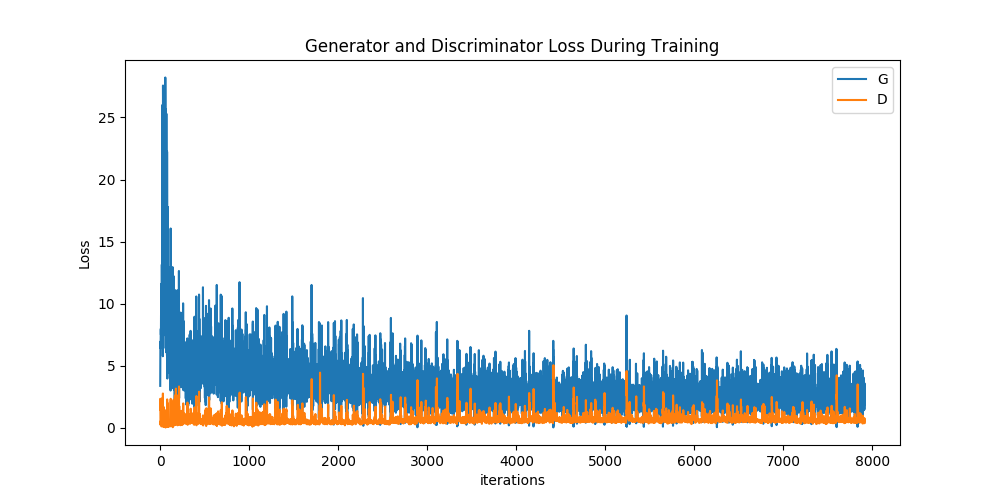
\includegraphics[totalheight=6cm]{Plot.png}
				\end{framed}
				\caption{Generator and Discriminator Loss During Training.}
			\end{figure}
		
			
			
		\subsection{Provide a Set of Real and Fake Images}
		 
		\begin{figure}
			\centering
			\begin{framed}
			\begin{subfigure}{.5\textwidth}
				\centering
				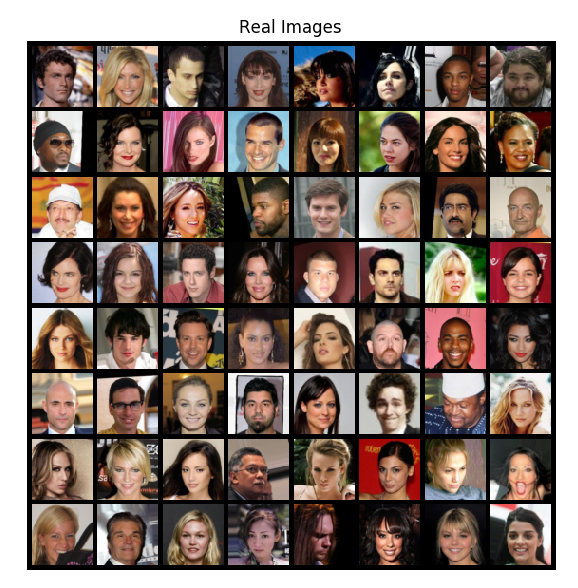
\includegraphics[width=7cm]{Real_Images_1.png}
				\caption{Set of real images.}
				\label{fig:sub1}
			\end{subfigure}%
			\begin{subfigure}{.5\textwidth}
				\centering
				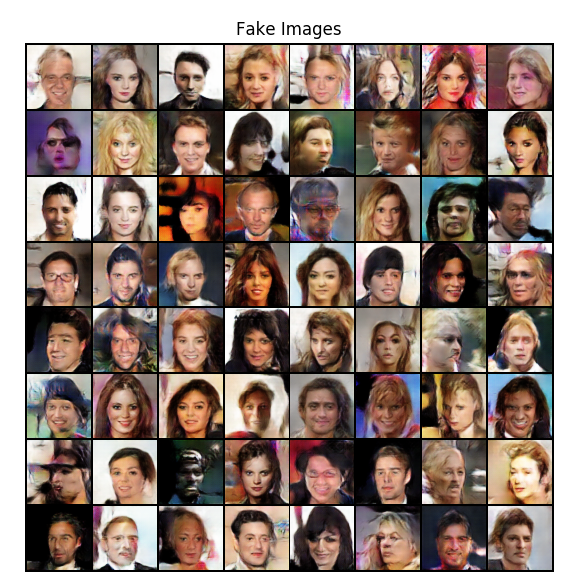
\includegraphics[width=7cm]{Fake_Images_1.png}
				\caption{Set of fake images.}
				\label{fig:sub2}
			\end{subfigure}
			\caption{A set of real and fake images}
			\label{fig:test}
			\end{framed}
		\end{figure}
		
	%\bibliographystyle{ieeetr}
	%\bibliography{references}
	
\end{document}
